\documentclass[14pt, aspectratio=169, handout]{beamer}
\usetheme{Copenhagen}
\usecolortheme{seahorse}
\setbeamertemplate{navigation symbols}{}
\setbeamertemplate{headline}{}

%\usepackage{pgfpages}
%\pgfpagesuselayout{4 on 1}[a4paper, border shrink=5mm]

\usepackage{graphicx} % Required for inserting images
\usepackage{multicol}
%\usepackage{enumitem}
\usepackage{amsfonts}
\usepackage{amsmath}
\usepackage{xcolor}
\definecolor{myblue}{RGB}{0, 0, 255} 
\definecolor{mygreen}{RGB}{0, 180, 80}
\definecolor{myred}{RGB}{153, 0, 0}
\definecolor{myorange}{RGB}{255, 153, 51}
\definecolor{mypurple}{RGB}{102, 0, 204}
\usepackage{tikz}

%--- commands for transform arrows----------------
\newcommand{\transform}[2]{%
    \begin{tikzpicture}
        % Open circle
        \draw[thick] (0,0) circle (0.1);
        % Line with number above and adjustable length
        \draw[thick] (0.1,0) -- (#2,0) node[midway, above] {#1};
        % Filled circle
        \filldraw[thick] (#2,0) circle (0.1);
    \end{tikzpicture}%
}
\newcommand{\invtransform}[2]{%
    \begin{tikzpicture}
        % filled circle
        \filldraw[thick] (0,0) circle (0.1);
        % Line with number above and adjustable length
        \draw[thick] (0.1,0) -- (#2 -0.1,0) node[midway, above] {#1};
        % open circle
        \draw[thick] (#2,0) circle (0.1);
    \end{tikzpicture}%
}
\newcommand{\verticaltransform}[4]{%
    \begin{tikzpicture}
        % Open circle at the bottom with text below
        \filldraw[thick] (0,0) circle (0.1) node[below=3pt] {$#4$};
        % Vertical line with number on the left
        \draw[thick] (0,0.1) -- (0,#2 -0.1) node[midway, left] {#1};
        % Filled circle at the top with text above
        \draw[thick] (0,#2) circle (0.1) node[above=3pt] {$#3$};
    \end{tikzpicture}%
}
\newcommand{\verticalinvtransform}[4]{%
    \begin{tikzpicture}
        % Open circle at the bottom with text below
        \draw[thick] (0,0) circle (0.1) node[below=3pt] {$#4$};
        % Vertical line with number on the left
        \draw[thick] (0,0.1) -- (0,#2) node[midway, left] {#1};
        % Filled circle at the top with text above
        \filldraw[thick] (0,#2) circle (0.1) node[above=3pt] {$#3$};
    \end{tikzpicture}%
}

\definecolor{darkblue}{RGB}{0, 0, 139}
\definecolor{lightblue}{RGB}{173, 216, 230}

\title{SST1 Übungsstunde 6}
\author{Matteo Dietz}
\date{November 2024}

\begin{document}

\maketitle

\begin{frame}{Themenüberblick}
    \begin{itemize}
        \item \textbf{Analoge Lineare Systeme im Frequenzbereich:}
        \item[] Kurze Repetition: Fouriertransformation und Eigenschaften
        \item[] Eigenfunktionen von LTI Systemen
        \item[] Antwort von LTI-Systemen im Frequenzbereich
        \item[] Kaskadierung von LTI-Systemen
    \end{itemize}
\end{frame}

\begin{frame}{Themenüberblick}
    \begin{itemize}
        \item \textbf{Spezielle Eingangssignale von LTI-Systemen}
        \item[] Allgemeine Schwingungen
        \item[] Sinusförmige Eingangssignale 
        \item[] Einschaltvorgänge
        \item[] Periodische Eingangssignale und Fourierreihen
        \item[] Deltakamm und Poissonsche Summenformel
    \end{itemize}
\end{frame}

\begin{frame}{Aufgaben für diese Woche}
    \begin{itemize}
        \item[] Dieselben wie letzte Woche und \textbf{69}, \textbf{70}, \textbf{71}, \textbf{72}, 73, \textbf{74}, 
        \item[] 
        \item[] Die \textbf{fettgedruckten} Übungen empfehle ich, weil sie wesentlich zu eurem Verständnis der Theorie beitragen und/oder sehr prüfungsrelevant sind.
    \end{itemize}
\end{frame}

\begin{frame}{Repetition: Eigenschaften der Fouriertransformation}
    \begin{itemize}
        \item \textbf{Definition}:
        \item[] 
        \item[] \fcolorbox{darkblue}{lightblue}{%
    \parbox{\dimexpr\linewidth-2\fboxsep-2\fboxrule\relax}{
    $$\text{(FT)} \hspace{20pt} \hat{x}(f) = (\mathcal{F}x)(f) = \int_{-\infty}^{\infty}x(t)e^{-2\pi i f t}\text{d}t$$
    $$\text{(IFT)} \hspace{10pt} x(t) = (\mathcal{F}^{-1}\hat{x})(t) = \int_{-\infty}^{\infty}\hat{x}(f)e^{2\pi i f t}\text{d}f$$
}}%
    \end{itemize}
\end{frame}

\begin{frame}{Riemann-Lebesgue Lemma}
    \begin{itemize}
        \item Es sei $x$ ein absolut integrierbares Signal, d.h. $x \in L^1$.
        \item[] 
        \item[]  Dann ist $(\mathcal{F}x)(f) = \hat{x}(f)$ stetig und $\displaystyle\lim_{|f| \to \infty} \hat{x}(f) = 0$.
    \end{itemize}
\end{frame}

\begin{frame}{Formelsammlung}
    \begin{center}
        \vspace*{-0.25cm}
        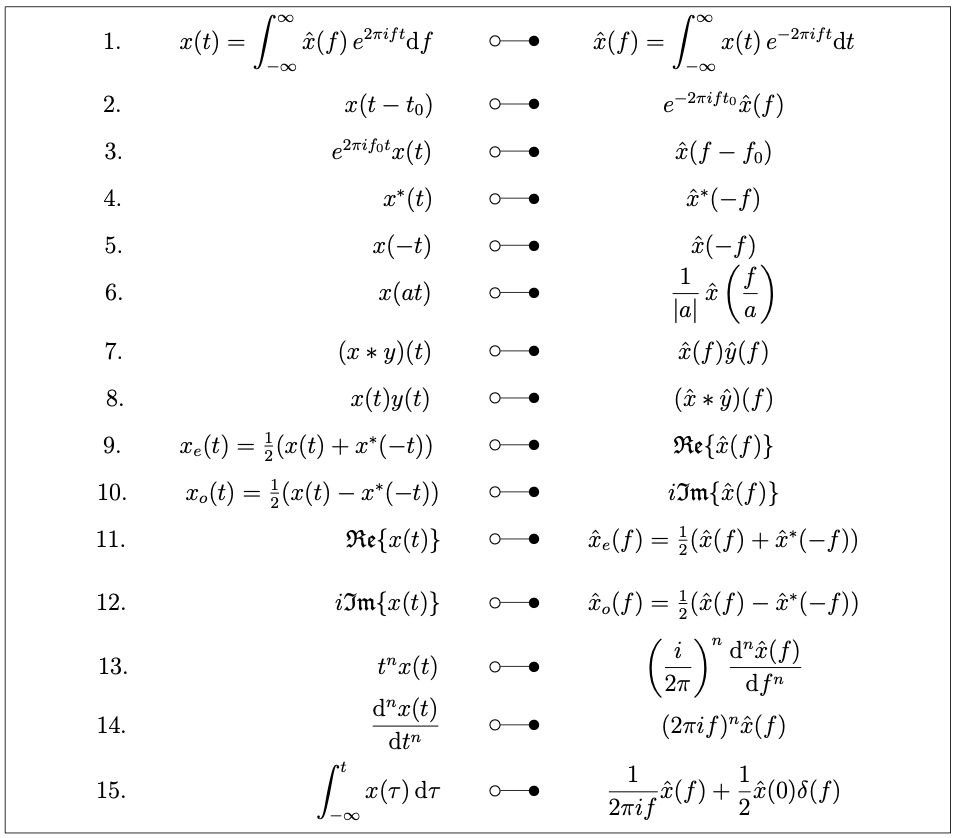
\includegraphics[width=0.6\linewidth]{figures/FT_eigenschaften.png}
    \end{center}
\end{frame}

\begin{frame}{Parseval und Plancherel}
    \fcolorbox{darkblue}{lightblue}{%
    \parbox{\dimexpr\linewidth-2\fboxsep-2\fboxrule\relax}{
    \begin{center}
        \textbf{Plancherelsche Identität:}
    \end{center}
    $$\langle x, y \rangle = \int_{-\infty}^{\infty} x(t)y^\ast (t)\text{d}t = \int_{-\infty}^{\infty}\hat{x}(f)\hat{y}^\ast(f)\text{d}f = \langle \hat{x}, \hat{y} \rangle$$
    \begin{center}
        \textbf{Parsevalsche Beziehung:}
    \end{center}
    $$||x||^2 = \langle x, x \rangle = \int_{-\infty}^{\infty} |x(t)|^2\text{d}t = \int_{-\infty}^{\infty}|\hat{x}(f)|^2\text{d}f = \langle \hat{x}, \hat{x} \rangle = ||\hat{x}||^2$$
    }}
\end{frame}

\begin{frame}{Aufgaben}
    \begin{itemize}
        \item \textbf{Aufgabe 66}
        \item[] 
        \item \textbf{Prüfungsaufgabe: Sommer 2019, Aufgabe 2}
    \end{itemize}
\end{frame}

\begin{frame}{Eigenfunktionen analoger LTI-Systeme}
    \begin{itemize}
        \item \textbf{Reminder}: Eigenvektoren $x$ sind Vektoren, die die Gleichung $Hx = \lambda x$ erfüllen, wobei $H$ ein System ist. $\lambda$ nennt man den dazugehörigen Eigenwert.
        \item[] 
        \item Wir wollen nun die Eigenfunktionen von analogen LTI Systemen finden. Das heisst, wir wollen $x(t)$ finden, sodass $y(t) = (Hx)(t) = \lambda x(t)$ gilt.
    \end{itemize}
\end{frame}

\begin{frame}{Eigenfunktionen analoger LTI-Systeme}
    \begin{itemize}
        \item \textbf{Eingangssignal}: $x(t)= e^{2\pi i f_0 t}$
        \item[] 
        \item[] Wir wenden nun darauf das LTI-System $H$ an:
        \begin{align*}
            y(t) &= (x \ast h)(t) = \int_{-\infty}^\infty x(t-\tau)h(\tau) \text{d}\tau \\
            &=\int_{-\infty}^\infty e^{2 \pi i f_0 (t-\tau)} h(\tau) \text{d}\tau = e^{2 \pi i f_0 t} \underbrace{\int_{-\infty}^\infty h(\tau) e^{-2\pi i f_0 \tau} \text{d}\tau}_{\hat{h}(f_0)} \\
            &\implies (He^{2 \pi i f_0 \cdot})(t) = \hat{h}(f_0)e^{2 \pi i f_0 t}
        \end{align*}
    \end{itemize}
\end{frame}

\begin{frame}{Eigenfunktionen analoger LTI-Systemen}
    $$\text{Es gilt also: } \hspace{12pt} (He^{2 \pi i f_0 \cdot})(t) = \hat{h}(f_0)e^{2 \pi i f_0 t}$$
    \vspace{0.25cm}
    \fcolorbox{darkblue}{lightblue}{\parbox{\dimexpr\linewidth-2\fboxsep-2\fboxrule\relax}{
        \textbf{Kunstgriff:}\\
        Die Funktionen $e^{2\pi i f_0 t}$ sind Eigenfunktionen von LTI-Systemen mit zugehörien Eigenwerten $\hat{h}(f_0)$
    }}%
\end{frame}

\begin{frame}{Antwort von LTI-Systemen im Frequenzbereich}
    
\end{frame}

\begin{frame}{Antwort von LTI-Systemen im Frequenzbereich}
    \begin{itemize}
        \item[] \fcolorbox{darkblue}{lightblue}{%
    \parbox{\dimexpr\linewidth-2\fboxsep-2\fboxrule\relax}{
    \begin{align*}
        (x \ast h)(t) \hspace{12pt} &\transform{7.}{2} \hspace{12pt} \hat{x}(f) \hat{h}(f) \\
        x(t)h(t) \hspace{12pt} &\transform{8.}{2} \hspace{12pt} (\hat{x} \ast \hat{h})(f)
    \end{align*}
    }}%
    \item[] 
    \item[] $\implies y(t) = (Hx)(t) = \displaystyle\int_{-\infty}^{\infty} \hat{x}(f) \hat{h}(f) e^{2 \pi i f t}\text{d}f$
    \item[] 
    \item[] 
    \item[] 
    \end{itemize}
\end{frame}

\begin{frame}{Blockschaltbilder}
    \begin{itemize}
        \item Wir können LTI-Systeme mit folgenden Blockschaltbildern beschreiben:
        \item[]
        \item[] \hspace{-0.25cm}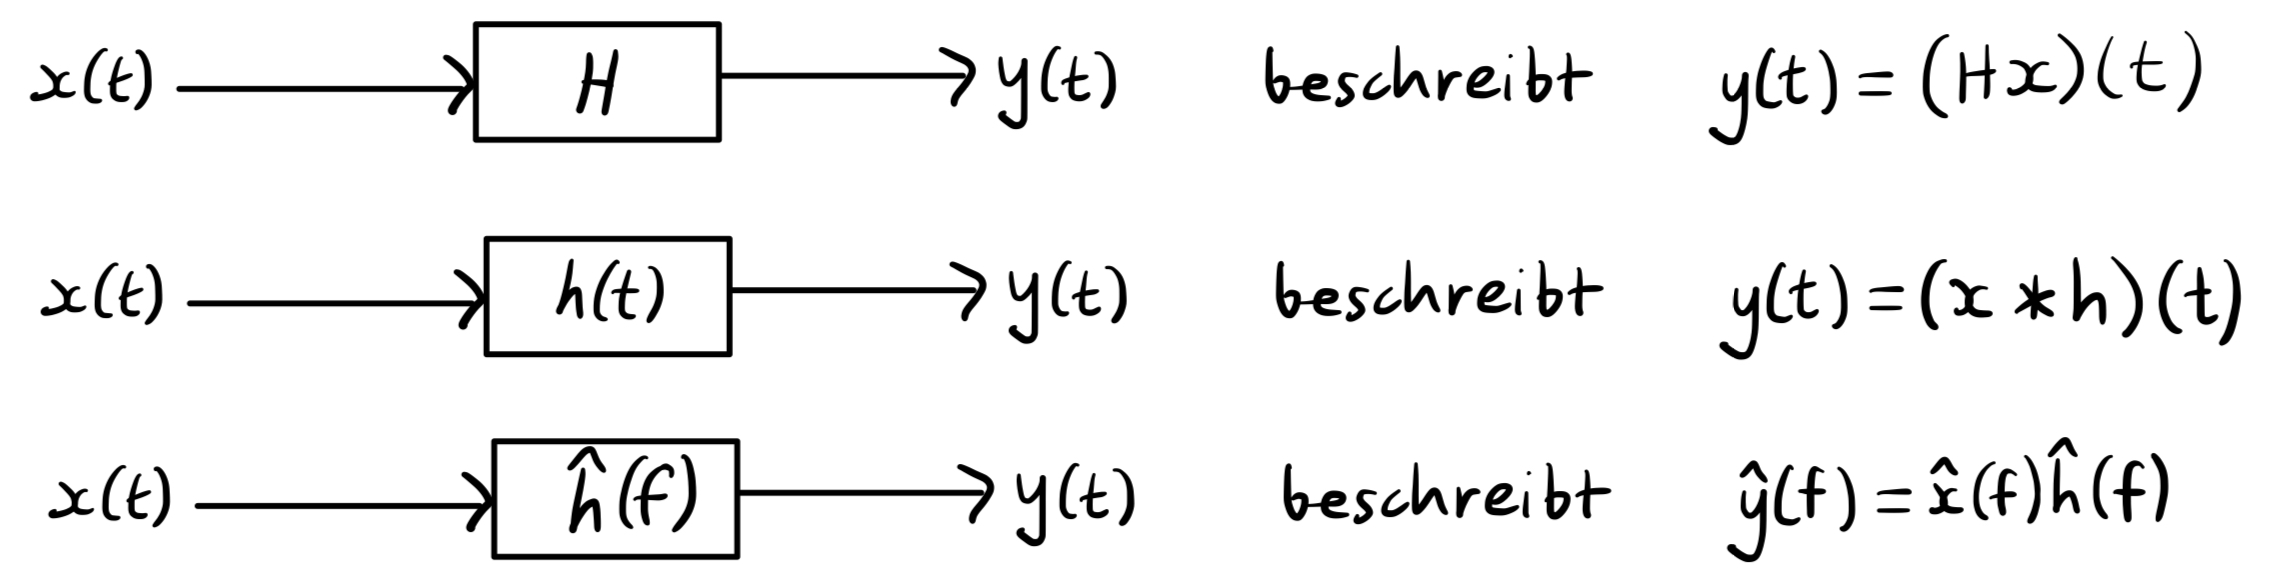
\includegraphics[width=\linewidth]{figures/Blockschaltilder.jpg}
    \end{itemize}
\end{frame}

\begin{frame}{Kaskadierung von LTI-Systemen}
    \begin{itemize}
        \item[] \begin{center}
            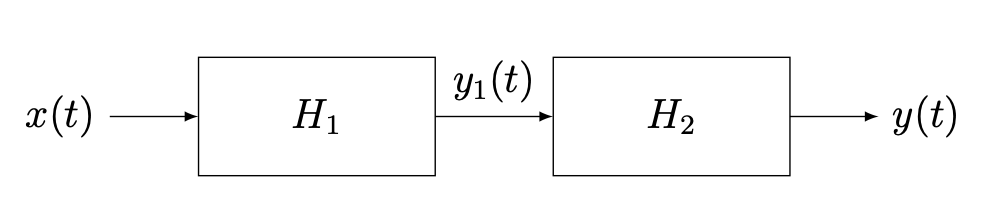
\includegraphics[width=\linewidth]{figures/Kaskadierung.png}
        \end{center}
        \item[] 
        \item[] \begin{center}
            \textbf{LTI-Systeme kommutieren}
        \end{center}
    \end{itemize}
\end{frame}

\begin{frame}{Kaskadierung von LTI-Systemen: Theorem}
    \begin{itemize}
        \item Es seien $A$ und $B$ zwei lineare Operatoren auf einem linearen Raum $V$ ausgestattet mit einem positiv definiten inneren Produkt. Dann sind die folgenden beiden Aussagen äquivalent: \begin{itemize}
        \item[] 
        \item[(i)] $A$ und $B$ besitzen eine gemeinsame Eigenbasis.
        \item[] 
        \item[(ii)] $A$ und $B$ kommutieren.
    \end{itemize}
    \item[] 
    \item LTI-Systeme haben die komplexen Exponentialfunktionen als gemeinsame Eigenbasis. Somit kommutieren LTI-Systeme.
    \end{itemize}
\end{frame}

\begin{frame}{Kaskadierung von LTI-Systemen}
    \begin{itemize}
        \item Kaskadierung der LTI-Systeme $H_1$ und $H_2$ mit $x=e^{2 \pi i f_0 t}$:
        \item[] 
        \item[] 
        \item[] 
        \item[] 
        \item[] 
        \item[] 
        \item[] 
        \item[] 
        \item[] \fcolorbox{darkblue}{lightblue}{%
    \parbox{\dimexpr\linewidth-2\fboxsep-2\fboxrule\relax}{
    Die Kaskadierung von LTI-Systemen ist wieder ein LTI-System mit $\hat{h}(f) = \hat{h}_1(f) \cdot \hat{h}_2(f)$ d.h. $h(t) = (h_1 \ast h_2)(t)$.
}}%
    \end{itemize}
\end{frame}

\begin{frame}{Spezielle Eingangssignale}
    \begin{itemize}
        \item \textbf{Allgemeine Schwingungen}
        \item[] 
        \item \textbf{Sinusförmige Eingangssignale}
        \item[] 
        \item \textbf{Einschaltvorgänge}
        \item[]
        \item \textbf{Allgemeine Periodische Signale}
    \end{itemize}
\end{frame}

\begin{frame}{Allgemeine Schwingungen}
    \begin{itemize}
        \item Eingangssignal $x(t) = \displaystyle e^{st}, \hspace{8pt} s \in \mathbb{C}$,
$ \hspace{8pt} \text{wobei }s = \sigma + i 2 \pi f_0, \hspace{12pt} \mathfrak{Re}(s) = \sigma \begin{cases}
    < 0, \\
    = 0, \\
    > 0,
\end{cases}$
    \item[] 
    \item[] dann $x(t) = \textcolor{myblue}{e^{\sigma t}}\textcolor{mygreen}{e^{i 2 \pi f_0 t}}, \hspace{12pt} \mathfrak{Re}(x(t)) = e^{\sigma t}\cos (2\pi f_0 t)$
    \item[] 
    \item $\textcolor{myblue}{e^{\sigma t}} =$ \textcolor{myblue}{Einhüllende} und $\textcolor{mygreen}{e^{i 2 \pi f_0 t}} =$ \textcolor{mygreen}{Schwingung}.
    \end{itemize}
\end{frame}

\begin{frame}{Allgemeine Schwingungen}
    \begin{itemize}
        \item Der Ausgang eines Systemes mit Impulsantwort $h(t)$ ist dann:
        \item[] 
        \item[] $y(t) = (x \ast h)(t) = \displaystyle\int_{-\infty}^{\infty} h(\tau)e^{s(t-\tau)} \text{d}\tau = e^{st} \underbrace{\int_{-\infty}^{\infty} h(\tau) e^{-s\tau} \text{d}\tau}_{=\text{H}(s)}$
        \item[] 
        \item[] $\text{H}(s) = \displaystyle\int_{-\infty}^{\infty} h(\tau) e^{-s\tau} \text{d}\tau=$ \textbf{Laplace-Transformierte} von $h(t)$.
    \end{itemize}
\end{frame}

\begin{frame}{Sinusförmige Eingangssignale}
    \begin{itemize}
    \item Eingangssignal: $x(t) = \cos(2 \pi f_0 t + \varphi_0) = \frac{1}{2} \displaystyle \textcolor{myblue}{e^{i 2 \pi f_0 t}} e^{i \varphi_0} + \frac{1}{2} \displaystyle \textcolor{myblue}{e^{-i 2 \pi f_0 t}} e^{-i \varphi_0}$
    \item[] 
    \item[] Ausgangssignal:
    \item[] $y(t) = (Hx)(t) = \frac{1}{2}\hat{h}(f_0)\displaystyle e^{i 2 \pi f_0 t} e^{i \varphi_0} + \frac{1}{2}\underbrace{\hat{h}(-f_0)}_{=\hat{h}^\ast (f_0)}e^{-i 2 \pi f_0 t} e^{-i \varphi_0}$
    \item[] $\hspace{30pt} = \frac{1}{2}\left(\hat{h}(f_0)e^{i 2 \pi f_0 t} e^{i \varphi_0} + \left(\hat{h}(f_0)e^{i 2 \pi f_0 t} \displaystyle e^{i \varphi_0}\right)^{\ast}\right)$
    \item[] $\hspace{30pt} = \displaystyle\mathfrak{Re}\left(  \hat{h}(f_0) e^{i 2 \pi f_0 t} e^{i \varphi_0} \right)$
    \end{itemize}
\end{frame}

\begin{frame}{Sinusförmige Eingangssignale}
    \begin{itemize}
        \item[] $\ \displaystyle\mathfrak{Re}\left(  \hat{h}(f_0) e^{i 2 \pi f_0 t} e^{i \varphi_0} \right) = \textcolor{myred}{|\hat{h}(f_0)|}\cdot \cos\left(\textcolor{mypurple}{2 \pi f_0 t} + \varphi_0 + \textcolor{myorange}{\text{arg}(\hat{h}(f_0))}\right)$, 
        \item[] 
        \item[] da $\hat{h}(f_0)$ komplexwertig sein kann.
        \item[] 
        \item Das Ausgangssignal auf ein sinusförmiges Eingangssignal ist ein \textcolor{myred}{skalierter} und \textcolor{myorange}{verschobener} Sinus, der mit \textcolor{mypurple}{derselben Frequenz} oszilliert wie das Eingangssignal.
    \end{itemize}
\end{frame}

\begin{frame}{Einschaltvorgänge}
    \begin{itemize}
    \item Eingangssignal: $x(t) = \displaystyle e^{2 \pi i f_0 t} \sigma(t) \hspace{15pt}$
    \item[] 
    \item Stationärer Zustand des Ausgangssignals $y(t) \displaystyle\xrightarrow{t \to \infty} \hat{h}(f_0) e^{2 \pi i f_0 t}$
    \item[] 
    \item Der Einschaltvorgang hat unendlich lange nach dem Einschalten keinen Einfluss mehr.
    \end{itemize}
\end{frame}

\begin{frame}{Fourierreihen: Definition}
    \fcolorbox{darkblue}{lightblue}{%
    \parbox{\dimexpr\linewidth-2\fboxsep-2\fboxrule\relax}{
        $$x(t) = x(t + T) = \sum_{k=-\infty}^{\infty} c_k e^{\frac{2 \pi i k t}{T}}, \hspace{12pt} \text{wobei} \hspace{12pt} c_k = \frac{1}{T}\int_0^T x(t) e^{-\frac{2 \pi i k t}{T}} \text{d}t$$
          \hspace{40pt} $x(t)$ wird gemäss Nr. 21 fouriertransformiert zu:
        $$(\mathcal{F}x)(f) = \hat{x}(f) = \mathcal{F}\left\{ \sum_{k = -\infty}^{\infty} c_k e^{\frac{2 \pi i k t}{T}}\right\} = \sum_{k = -\infty}^{\infty} c_k \delta\left( f - \frac{k}{T} \right)$$
    }}%
\end{frame}

\begin{frame}{Fourierreihen: Eigenschaften}
    \begin{itemize}
        \item[(i)] Fourierreihen existieren nur für periodische Signale.
        \item[] 
        \item[(ii)] Periodische Signale haben immer ein "diskretes" Frequenzspektrum.
        \item[] 
        \item[(iii)] $c_k$ sind die komplexen Koeffizienten und beschreiben das Signal im Frequenzbereich.
    \end{itemize}
\end{frame}

\begin{frame}{Fourierreihen: Eigenschaften}
    \begin{itemize}
        \item Wir schreiben $x(t) = x(t+T) \; \transform{}{1} \; c_k$
        \item[] 
        \item Die $c_k$ beschreiben die Gewichte des Deltakamms.
        \item[]
        \item[] \begin{center}
            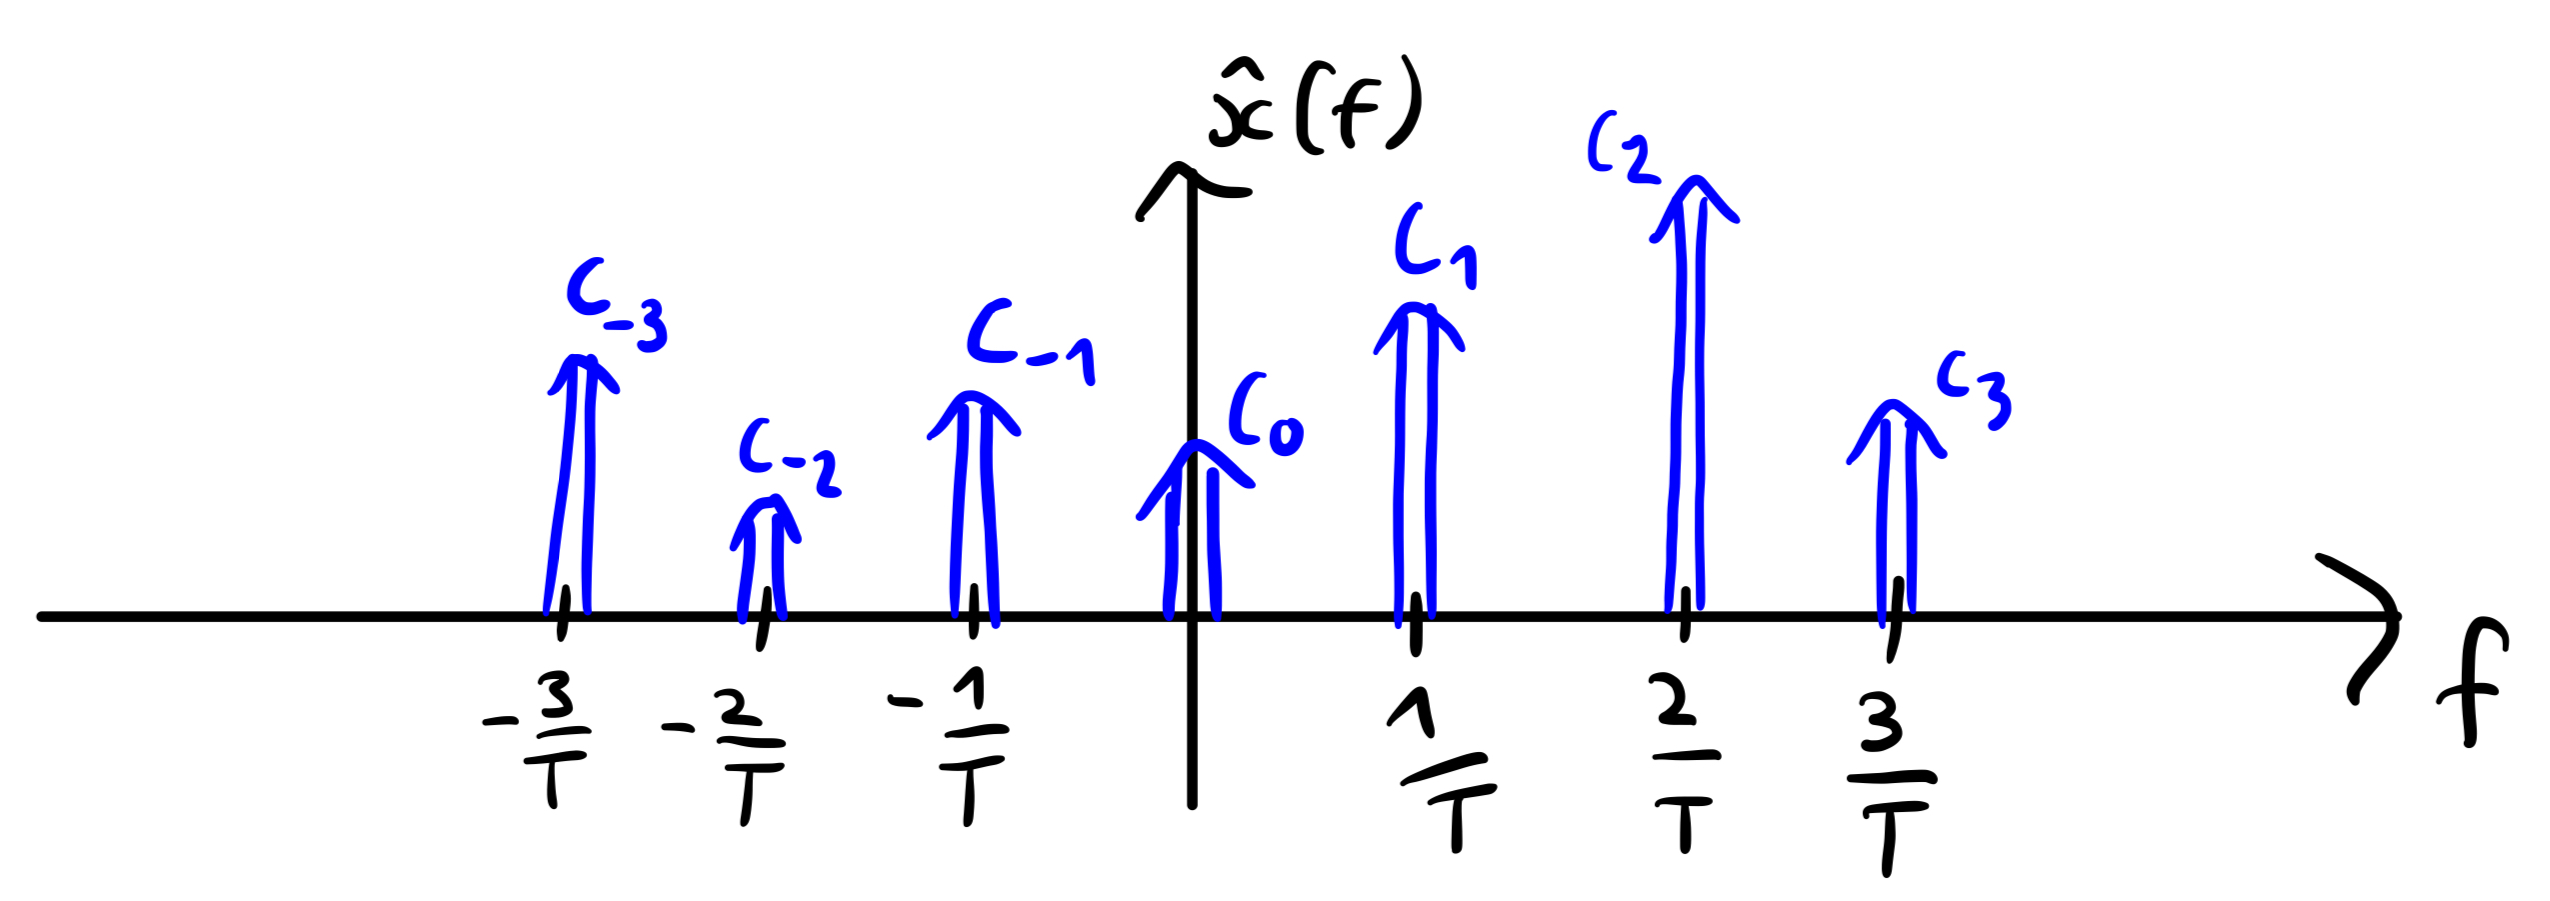
\includegraphics[width=0.7\linewidth]{figures/delta_gewichtet.jpg}
        \end{center}
    \end{itemize}
\end{frame}

\begin{frame}{Fourierreihen: Eigenschaften}
    \begin{itemize}
         \item Eigentlich ist das Spektrum kontinuierlich, es hat jedoch nur an Vielfachen von $1/T$ Komponenten, die ungleich null sind.
        \item[] \begin{center}
            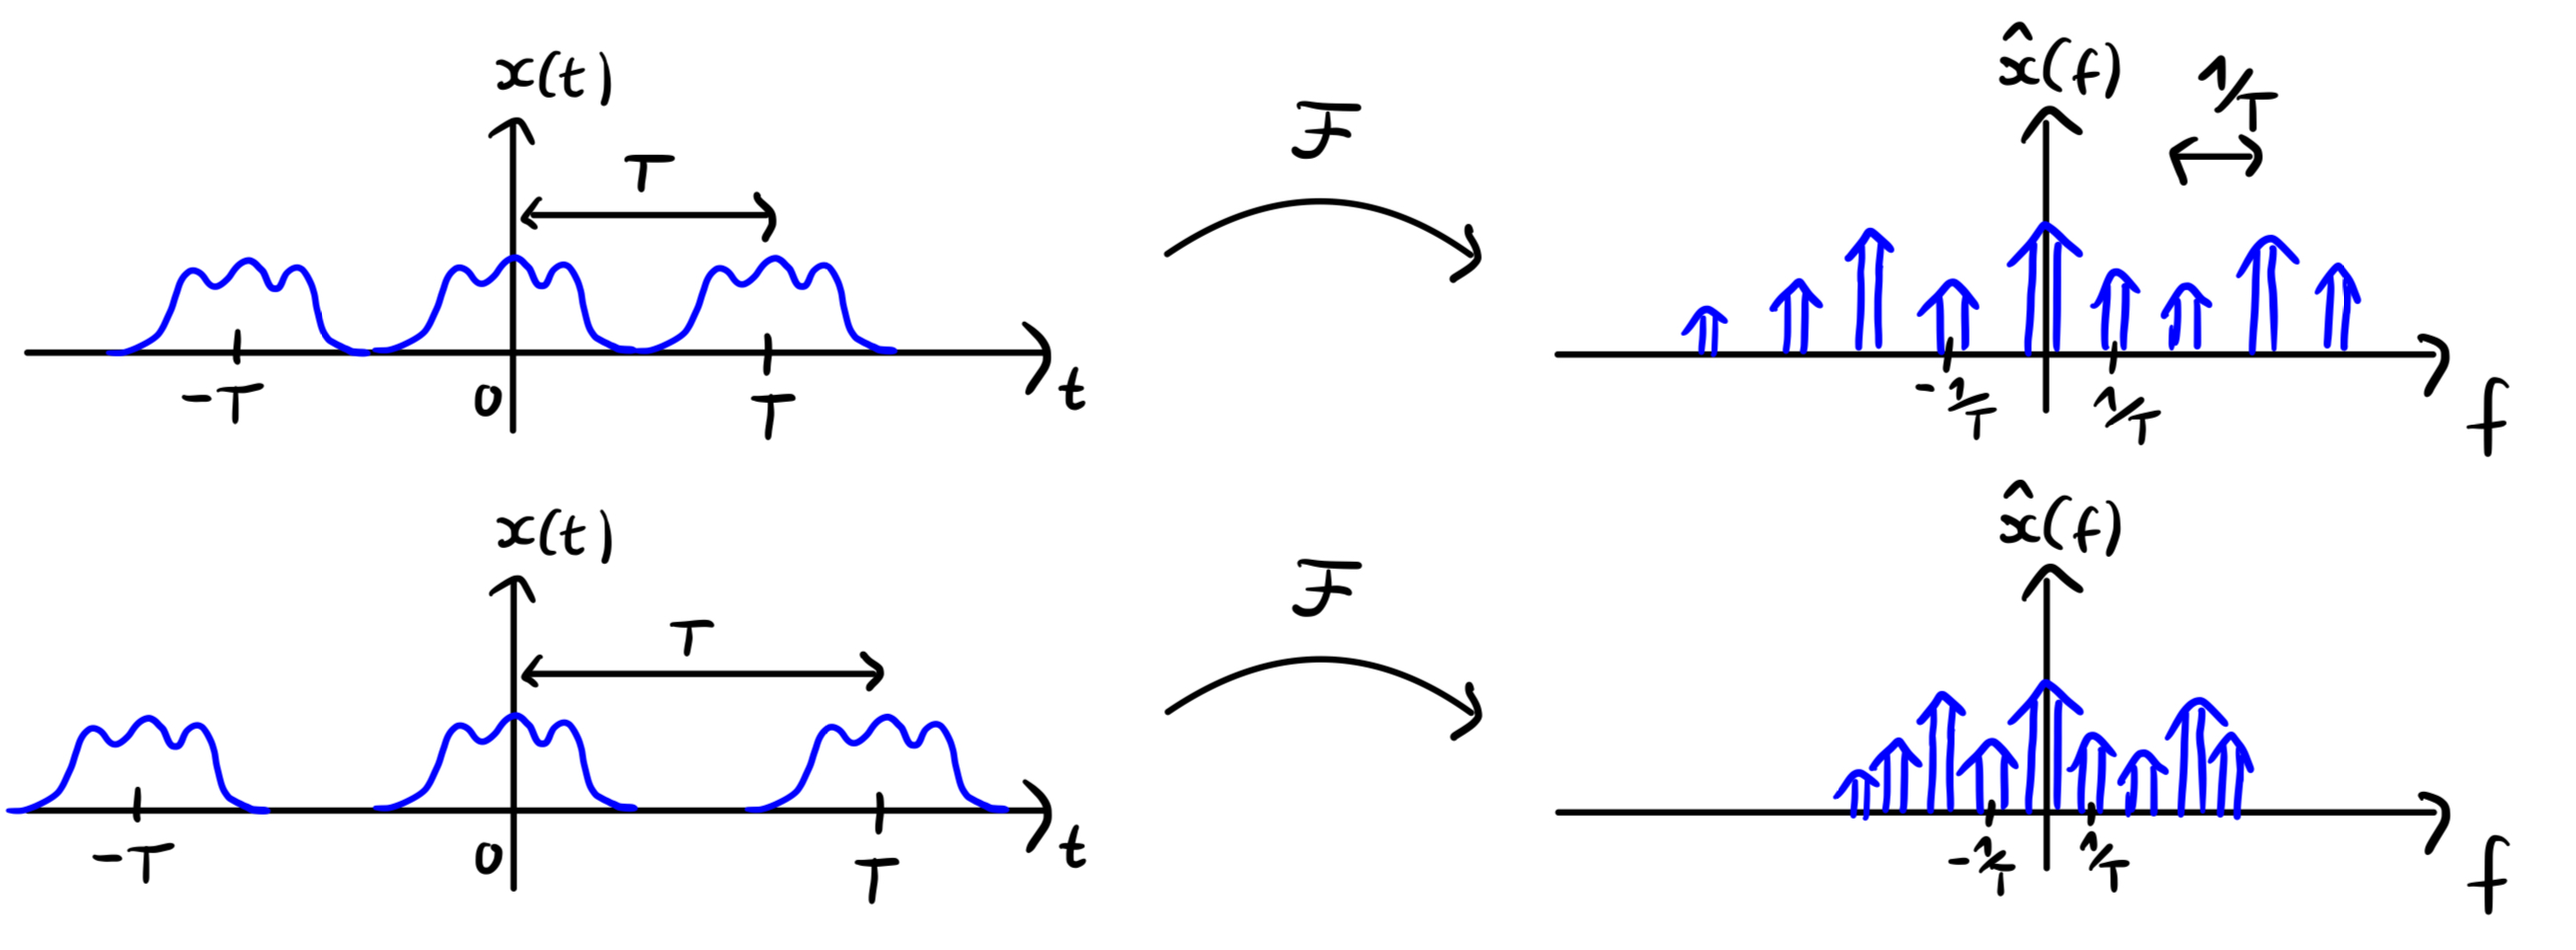
\includegraphics[width=0.8\linewidth]{figures/T_increase.jpg}
        \end{center}
        \item $1/T \xrightarrow{T \to \infty} 0$ somit wird die Fourierreihe zu einem Integral. Das "diskrete" Spektrum wird kontinuierlich.
    \end{itemize}
\end{frame}

\begin{frame}{Periodische Signale an LTI-Systemen}
    \begin{itemize}
        \item[] Eingangssignal: $x(t) = \displaystyle\sum_{k = -\infty}^{\infty} c_k e^{\frac{2 \pi i k t}{T}}$
        \item[] 
        \item[] Zur Erinnerung: $\left(H \displaystyle e^{2 \pi i f_0 \cdot}\right)(t) = \hat{h}(f_0) e^{2 \pi i f_0 t}$
        \item[] 
        \item[] Dank Linearität und Stetigkeit gilt:
        \item[] $\left(H x\right)(t) = \left(H \displaystyle\sum_{k = -\infty}^{\infty} c_k e^{\frac{2 \pi i k \cdot}{T}}\right)(t) = \displaystyle\sum_{k = -\infty}^{\infty} c_k \left(He^{\frac{2 \pi i k \cdot}{T}}\right)(t)$
    \end{itemize}
\end{frame}

\begin{frame}{Periodische Signale an LTI-Systemen}
    \fcolorbox{darkblue}{lightblue}{%
    \parbox{\dimexpr\linewidth-2\fboxsep-2\fboxrule\relax}{
        $$\hspace{-30pt} \implies y(t) = (Hx)(t) = \sum_{k = -\infty}^{\infty} \smash{\underbrace{c_k \hat{h}\left(\frac{k}{T}\right)}_{d_k}} e^{\frac{2 \pi i k t}{T}}$$
        \vspace*{0.15cm}
    }}%
    \begin{itemize}
    \item[] 
    \item Das Ausgangssignal auf ein $T-$periodisches Eingangssignal ist auch $T-$periodisch.
    \end{itemize}
\end{frame}

\begin{frame}{Deltakamm}
    Ein Deltakamm ist definiert durch:
    $$\delta_T(t) = \sum_{k = -\infty}^{\infty} \delta(t-kT) \hspace{8pt} \transform{51.}{1.5} \hspace{8pt} c_k = \frac{1}{T} \hspace{12pt} \forall k \in \mathbb{Z}$$
    Antwort eines LTI-Systems auf einen Deltakamm $\delta_T(t)$:
    \begin{align*}
        y(t) &\overset{\text{LTI}}{=} (h \ast \delta_T)(t) = \left(h \ast \sum_{k = -\infty}^\infty \delta(\cdot - kT) \right)(t) \\
        &\overset{\text{LIN}}{=} \sum_{k = -\infty}^\infty \left(h \ast \delta(\cdot - kT)\right)(t) = \sum_{k = -\infty}^\infty h(t-kT)
    \end{align*}
\end{frame}

\begin{frame}{Poissonsche Summenformel}
    \begin{itemize}
        \item LTI-Systeme antworten auf das Eingangssignal $x(t) = \delta_T(t)$ mit $y(t) = \displaystyle\sum_{k = -\infty}^\infty h(t-kT)$
        \item[] 
        \item[] 
        \item[] 
        \item[] 
        \item[] 
        \item $y(t)$ ist $T-$periodisch und kann somit als Fourierreihe $y(t) = \displaystyle\sum_{k = -\infty}^\infty d_k e^{\frac{2 \pi i k t}{T}}$ entwickelt werden.
    \end{itemize}
\end{frame}

\begin{frame}{Poissonsche Summenformel}
\begin{itemize}
    \item Dank $x(t) \; \transform{51.}{1} \; \frac{1}{T} \; \forall k \in \mathbb{Z}$  und $d_k = c_k \hat{h}\left(\frac{k}{T}\right)$ erhalten wir:
    \item[] 
\end{itemize} 
\fcolorbox{darkblue}{lightblue}{%
    \parbox{\dimexpr\linewidth-2\fboxsep-2\fboxrule\relax}{
        $$\hspace{12pt} \sum_{-\infty}^\infty h(t-kT) = \frac{1}{T} \sum_{-\infty}^\infty \hat{h}\left(\frac{k}{T}\right)e^{\frac{2\pi i k t}{T}}
        $$
    }}%
\end{frame}

\begin{frame}{Aufgaben}
    \begin{itemize}
        \item \textbf{Prüfungsaufgabe: Frühjahr 2024, Aufgabe 1.a)ii, iii, iv und 1.d)i, ii}
    \end{itemize}
\end{frame}

\end{document}
